\documentclass[margin=0mm]{standalone}
\usepackage{tikz}
\usepackage{pgfplots}
 \pgfplotsset{compat=newest}

\usepackage{tikzorbital}

\begin{document}

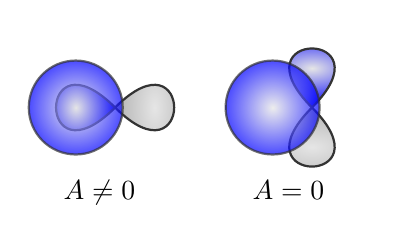
\begin{tikzpicture} 


\orbital[pos = {(3.5,0)}]{pz}

\orbital[pos = {(3,0)}, scale=2, opacity=0.7]{s}


\orbital[pos = {(1,0)}]{-py}

\orbital[pos = {(0.5,0)}, scale=2, opacity=0.7]{s}

\node[below] at (0.8,-0.8) {$A \neq 0$};
\node[below] at (3.2,-0.8) {$A = 0$};


\end{tikzpicture}



\end{document}